%%%%%%%%%%%%%%%%%%%%%%%%%%%%%%%%%%%%%%%%%
% Masters/Doctoral Thesis 
% LaTeX Template
% Version 1.43 (17/5/14)
%
% This template has been downloaded from:
% http://www.LaTeXTemplates.com
%
% Original authors:
% Steven Gunn 
% http://users.ecs.soton.ac.uk/srg/softwaretools/document/templates/
% and
% Sunil Patel
% http://www.sunilpatel.co.uk/thesis-template/
%
% License:
% CC BY-NC-SA 3.0 (http://creativecommons.org/licenses/by-nc-sa/3.0/)
%
% Note:
% Make sure to edit document variables in the Thesis.cls file
%
%%%%%%%%%%%%%%%%%%%%%%%%%%%%%%%%%%%%%%%%%

%----------------------------------------------------------------------------------------
%	PACKAGES AND OTHER DOCUMENT CONFIGURATIONS
%----------------------------------------------------------------------------------------

\documentclass[11pt, oneside]{Thesis} % The default font size and one-sided printing (no margin offsets)

\graphicspath{{Pictures/}} % Specifies the directory where pictures are stored

\usepackage[square, numbers, comma, sort&compress]{natbib} % Use the natbib reference package - read up on this to edit the reference style; if you want text (e.g. Smith et al., 2012) for the in-text references (instead of numbers), remove 'numbers' 
\usepackage{hyperref}
\hypersetup{urlcolor=black, colorlinks=true} % Colors hyperlinks in blue - change to black if annoying
\title{\ttitle} % Defines the thesis title - don't touch this

\begin{document}

\frontmatter % Use roman page numbering style (i, ii, iii, iv...) for the pre-content pages

\setstretch{1.3} % Line spacing of 1.3

% Define the page headers using the FancyHdr package and set up for one-sided printing
\fancyhead{} % Clears all page headers and footers
\rhead{\thepage} % Sets the right side header to show the page number
\lhead{} % Clears the left side page header

\pagestyle{fancy} % Finally, use the "fancy" page style to implement the FancyHdr headers

\newcommand{\HRule}{\rule{\linewidth}{0.5mm}} % New command to make the lines in the title page

% PDF meta-data
\hypersetup{pdftitle={\ttitle}}
\hypersetup{pdfsubject=\subjectname}
\hypersetup{pdfauthor=\authornames}
\hypersetup{pdfkeywords=\keywordnames}

%----------------------------------------------------------------------------------------
%	TITLE PAGE
%----------------------------------------------------------------------------------------

\begin{titlepage}
\begin{center}

\textsc{\LARGE \univname}\\[1.5cm] % University name
\textsc{\Large Master's thesis}\\[0.5cm] % Thesis type

\HRule \\[0.4cm] % Horizontal line
{\huge \bfseries \ttitle}\\[0.4cm] % Thesis title
\HRule \\[1.5cm] % Horizontal line
 
\begin{minipage}{0.4\textwidth}
\begin{flushleft} \large
\emph{Author:}\\
{\authornames} % Author name - remove the \href bracket to remove the link
\end{flushleft}
\end{minipage}
\begin{minipage}{0.4\textwidth}
\begin{flushright} \large
\emph{Supervisor:} \\
{\supname} % Supervisor name - remove the \href bracket to remove the link  
\end{flushright}
\end{minipage}\\[3cm]
 
\deptname\\[2cm] % Research group name and department name
 
{\large \today}\\[4cm] % Date
%\includegraphics{Logo} % University/department logo - uncomment to place it
 
\vfill
\end{center}

\end{titlepage}

%----------------------------------------------------------------------------------------
%	DECLARATION PAGE
%	Your institution may give you a different text to place here
%----------------------------------------------------------------------------------------

%\Declaration{
%
%\addtocontents{toc}{\vspace{1em}} % Add a gap in the Contents, for aesthetics
%
%I, \authornames, declare that this thesis titled, '\ttitle' and the work presented in it are my own. I confirm that:
%
%\begin{itemize} 
%\item[\tiny{$\blacksquare$}] This work was done wholly or mainly while in candidature for a research degree at this University.
%\item[\tiny{$\blacksquare$}] Where any part of this thesis has previously been submitted for a degree or any other qualification at this University or any other institution, this has been clearly stated.
%\item[\tiny{$\blacksquare$}] Where I have consulted the published work of others, this is always clearly attributed.
%\item[\tiny{$\blacksquare$}] Where I have quoted from the work of others, the source is always given. With the exception of such quotations, this thesis is entirely my own work.
%\item[\tiny{$\blacksquare$}] I have acknowledged all main sources of help.
%\item[\tiny{$\blacksquare$}] Where the thesis is based on work done by myself jointly with others, I have made clear exactly what was done by others and what I have contributed myself.\\
%\end{itemize}
% 
%Signed:\\
%\rule[1em]{25em}{0.5pt} % This prints a line for the signature
% 
%Date:\\
%\rule[1em]{25em}{0.5pt} % This prints a line to write the date
%}
%
%\clearpage % Start a new page

%----------------------------------------------------------------------------------------
%	QUOTATION PAGE
%----------------------------------------------------------------------------------------

%\pagestyle{empty} % No headers or footers for the following pages
%
%\null\vfill % Add some space to move the quote down the page a bit
%
%\textit{``Thanks to my solid academic training, today I can write hundreds of words on virtually any topic without possessing a shred of information, which is how I got a good job in journalism."}
%
%\begin{flushright}
%Dave Barry
%\end{flushright}
%
%\vfill\vfill\vfill\vfill\vfill\vfill\null % Add some space at the bottom to position the quote just right
%
%\clearpage % Start a new page

%----------------------------------------------------------------------------------------
%	ABSTRACT PAGE
%----------------------------------------------------------------------------------------

%\addtotoc{Abstract} % Add the "Abstract" page entry to the Contents
%
%\abstract{\addtocontents{toc}{\vspace{1em}} % Add a gap in the Contents, for aesthetics
%
%The Thesis Abstract is written here (and usually kept to just this page). The page is kept centered vertically so can expand into the blank space above the title too\ldots
%}
%
%\clearpage % Start a new page

%----------------------------------------------------------------------------------------
%	ACKNOWLEDGEMENTS
%----------------------------------------------------------------------------------------

%\setstretch{1.3} % Reset the line-spacing to 1.3 for body text (if it has changed)
%
%\acknowledgements{\addtocontents{toc}{\vspace{1em}} % Add a gap in the Contents, for aesthetics
%
%The acknowledgements and the people to thank go here, don't forget to include your project advisor\ldots
%}
%\clearpage % Start a new page

%----------------------------------------------------------------------------------------
%	LIST OF CONTENTS/FIGURES/TABLES PAGES
%----------------------------------------------------------------------------------------

\pagestyle{fancy} % The page style headers have been "empty" all this time, now use the "fancy" headers as defined before to bring them back

\lhead{\emph{Contents}} % Set the left side page header to "Contents"
\tableofcontents % Write out the Table of Contents

%    \lhead{\emph{List of Figures}} % Set the left side page header to "List of Figures"
%    \listoffigures % Write out the List of Figures
%    
%    \lhead{\emph{List of Tables}} % Set the left side page header to "List of Tables"
%    \listoftables % Write out the List of Tables

%----------------------------------------------------------------------------------------
%	ABBREVIATIONS
%----------------------------------------------------------------------------------------

%\clearpage % Start a new page
%
%\setstretch{1.5} % Set the line spacing to 1.5, this makes the following tables easier to read
%
%\lhead{\emph{Abbreviations}} % Set the left side page header to "Abbreviations"
%\listofsymbols{ll} % Include a list of Abbreviations (a table of two columns)
%{
%\textbf{LAH} & \textbf{L}ist \textbf{A}bbreviations \textbf{H}ere \\
%%\textbf{Acronym} & \textbf{W}hat (it) \textbf{S}tands \textbf{F}or \\
%}

%----------------------------------------------------------------------------------------
%	PHYSICAL CONSTANTS/OTHER DEFINITIONS
%----------------------------------------------------------------------------------------

%\clearpage % Start a new page
%
%\lhead{\emph{Physical Constants}} % Set the left side page header to "Physical Constants"
%
%\listofconstants{lrcl} % Include a list of Physical Constants (a four column table)
%{
%Speed of Light & $c$ & $=$ & $2.997\ 924\ 58\times10^{8}\ \mbox{ms}^{-\mbox{s}}$ (exact)\\
%% Constant Name & Symbol & = & Constant Value (with units) \\
%}

%----------------------------------------------------------------------------------------
%	SYMBOLS
%----------------------------------------------------------------------------------------

%\clearpage % Start a new page
%
%\lhead{\emph{Symbols}} % Set the left side page header to "Symbols"
%
%\listofnomenclature{lll} % Include a list of Symbols (a three column table)
%{
%$a$ & distance & m \\
%$P$ & power & W (Js$^{-1}$) \\
%% Symbol & Name & Unit \\
%
%& & \\ % Gap to separate the Roman symbols from the Greek
%
%$\omega$ & angular frequency & rads$^{-1}$ \\
%% Symbol & Name & Unit \\
%}

%----------------------------------------------------------------------------------------
%	DEDICATION
%----------------------------------------------------------------------------------------

%\setstretch{1.3} % Return the line spacing back to 1.3
%
%\pagestyle{empty} % Page style needs to be empty for this page
%
%\dedicatory{For/Dedicated to/To my\ldots} % Dedication text
%
%\addtocontents{toc}{\vspace{2em}} % Add a gap in the Contents, for aesthetics

%----------------------------------------------------------------------------------------
%	THESIS CONTENT - CHAPTERS
%----------------------------------------------------------------------------------------

\mainmatter % Begin numeric (1,2,3...) page numbering

\pagestyle{fancy} % Return the page headers back to the "fancy" style

% Include the chapters of the thesis as separate files from the Chapters folder
% Uncomment the lines as you write the chapters

% Chapter 1

\chapter{Introduction} % Main chapter title

\label{Intro} % For referencing the chapter elsewhere, use \ref{Chapter1} 

\lhead{\emph{Introduction}} % This is for the header on each page - perhaps a shortened title

\section{Similarity of data}

How do we know that Dutch is more similar to German than it is to French? How do we know that Bob Dylan's music is closer to The Beatles' than it is to Bach's?

Does a computer know? 

This thesis concerns a method expressing similarity of data that is feature free: it does not use domain knowledge about the data (for example, word origins or grammar rules in the case of languages.) The method is based on file compression and is rooted in Kolmogorov complexity.

The idea is easy to grasp. If a compressor compresses the concatenation of two files better than it compresses the files separately, it must have found some regularities that appear in both files. This compression gain is used to define a similarity metric that aims to capture the similarity of every dominant feature of the data.

% Chapter Template

\chapter{Normalized compression distance} % Main chapter title

\label{Chapter2} % Change X to a consecutive number; for referencing this chapter elsewhere, use \ref{ChapterX}

\lhead{Chapter 2. \emph{Normalized compression distance}} % Change X to a consecutive number; this is for the header on each page - perhaps a shortened title

\section{Foundations in Kolmogorov complexity}

In this chapter we will make explicit the idea of similarity based on file compression. But first, we explain the notion of Kolmogorov complexity. For a complete reference, see \cite{li2009introduction}.

The Kolmogorov complexity of a string $x$, written $K(x)$, is the length of the shortest program that outputs $x$.

Intuitively, $111\dots111$, a string of a million ones, is not very complex. It does not contain much information. Indeed, the Kolmogorov complexity of this string is low. A 27-byte Ruby program produces it:

\begin{verbatim}
1000000.times { print "1" }
\end{verbatim}

I do not claim the Kolmogorov complexity of a string of a million ones is 27 bytes. The true Kolmogorov complexity of a string $x$ cannot be computed in the Turing sense. There is no program that, given $x$, outputs the (length of) the shortest program that produces $x$.

The string $011\dots010$, produced by flipping a fair coin a million times, has, with very high probability, a Kolmogorov complexity close to its own length (by counting the number of different bit strings of each length, you can show that the chance to compress a random string by more than $c$ bits is at most $2^{-c}$).

So, printing the literal description may be the best we can do:

\begin{verbatim}
print "011...010"
\end{verbatim}

The Kolmogorov complexity of a string $x$, given a string $y$, denoted by $K(x|y)$, is the length of the shortest program that outputs $x$, given $y$ as input.

\subsection{The Kolmogorov complexity is not computable}

To prove that $K(x)$ is not computable, suppose there is a program \lstinline{kolmogorov_complexity(x)} that computes $K(x)$. Now consider the following program, that outputs a string $x$ with $K(x) \geq n$.

\begin{lstlisting}[frame=single]
def p(n)
  all_strings_of_length(n).each do |x|
    if kolmogorov_complexity(x) >= n
      return x
    end
  end
end
\end{lstlisting}

Encoding $x$ with $p(n)$ takes only $c + 2log(n)$ bits: a constant number of bits for the programs \lstinline{kolmogorov_complexity(x)} and \lstinline{p(n)}, and $2log(n)$ to encode $n$. Since there exist strings with arbitrarily large Kolmogorov complexity, this is a contradiction, hence $K(x)$ is not computable.

\subsection{Information distance}

The Kolmogorov complexity is a measure of information content in an individual object. In the same way, in \cite{Bennett1998} the information distance $E(x, y)$ between two strings $x$ and $y$ is defined as the length of the shortest program that converts $x$ to $y$ and $y$ to $x$. It is shown that

$$ E(x, y) = \max \{ K(x|y), K(y|x) \} $$

$E(x, y)$ is an absolute distance. But similarity is better expressed relatively. To illustrate: if two binary strings of length 100 have a Hamming distance of 50 (i.e. they have different bits in 50 positions), they are not very alike. If, on the other hand, two strings of length $10^{6}$ have a Hamming distance of 50, they are very much alike.

In \cite{Li2004}, the normalized information distance is defined as

\begin{equation}\label{nid}
  \text{NID}(x, y) = \frac{\max \{ K(x|y), K(y|x) \}}{\max \{ K(x), K(y)\}}
\end{equation}

and it is shown that $ \text{NID}(x, y)$ minorizes every distance $d(x, y)$ up to a negligible additive term, where $d(x, y)$ belongs to a wide class of normalized distances that includes everything remotely interesting.

This means that if two strings are similar according to some distance (be it Hamming distance, overlap distance, or any other), they are also similar according to the normalized information distance. This is why $	\text{NID}(x, y)$ is also called \emph{the} similarity distance.

\section{Approximating Kolmogorov complexity with a real-world compressor}

The remarkable properties of the normalized information distance come at the price of incomputability. But, the Kolmogorov complexity can be approximated by real-world (lossless) compression programs like zlib or liblzma. The normalized compression distance \cite{Cilibrasi2005} is defined as

\begin{equation}\label{ncd}
  \text{NCD} = \frac{C(xy) - \min \{ C(x), C(y) \}}{\max \{ C(x), C(y) \}}
\end{equation}

where $xy$ is the concatenation of $x$ and $y$, and $C(x)$ is the length of $x$, after being compressed by compressor $C$.

The $\text{NCD}$ is central to this work. It is the real-world approximation of the normalized information distance \eqref{nid}.

The authors of \cite{Cilibrasi2005} show that most (if not all) real-world compressors guarantee that the NCD is a quasi-universal similarity metric, by satisfying the following properties:

\begin{enumerate}
  \item \emph{idempotency}: $C(xx) = C(x)$
  \item \emph{monotonicity}: $C(xy) \geq C(x)$
  \item \emph{symmetry}: $C(xy) = C(yx)$
  \item \emph{distributivity}: $C(xy) + C(z) \leq C(xz) + C(yz)$
\end{enumerate}

\subsection{A compressor does not exploit all regularity}
Since $K$ is incomputable, we have no idea how far off the length given by $C$ is. Consider $31415...$, the string consisting of the first $10^{9}$ digits of $\pi$. The Kolmogorov complexity of this string is low: a simple program, perhaps exploiting a converging series formula, will produce it. Any real-world compressor $C$, however, fails to compress this string by even a few bits\footnote{A textual representation "31415..." can actually be compressed significantly by almost every compressor, but this is an encoding issue. The file consists only of the bytes 0 through 9, which can be more efficiently encoded using, for example, a system where each decimal number is assigned a four bit code (which is still naive.) For clarity, I do not concern myself with encoding in this chapter. Every finite alphabet can be recoded in binary, so it is customary to only think about binary strings in the literature. Conceptually, nothing changes. }.

In the following chapters (and extensively in \cite{Cilibrasi2005}) it is demonstrated that, while not every regularity is captured by a real-world compressor, the $\text{NCD}$ is still adequate for many applications.
 
% Chapter Template

\chapter{Hierarchical clustering of data}
% Main chapter title

\label{Chapter3} % Change X to a consecutive number; for referencing this chapter elsewhere, use \ref{ChapterX}

\lhead{Chapter 3. \emph{Hierarchical clustering of data}} 

In this chapter, we cluster vastly different types of data using the
normalized compression distance (NCD) \eqref{ncd}. To explain the method,
we first cluster mitochondrial gene sequences of mammals.

\section{Evolution of placental mammals}

Reconstructing an evolutionary tree has intuitive appeal. It should lend
itself well to hierarchical clustering, since species emerge from common
ancestors. And, within biology, there is agreement on what the true
phylogeny tree is: the brown bear and polar bear are closely related, etc.
Only higher up on the tree there is ongoing debate. Do the primates first
join with the rodents, or are they more closely connected to the
ferungulates? 

All materials were taken from the GenBank database \cite{GenBank}.

In \cite{Cao1998}, the authors estimate the likelihood of phylogeny trees
based on 12 mitochondrial proteins of 20 placental mammals: rat
(\emph{Rattus norvegicus}), house mouse (\emph{Mus musculus}), grey seal
(\emph{Halichoerus grypus}), harbor seal (\emph{Phoca vitulina}), cat
(\emph{Felis catus}), white rhino (\emph{Ceratotherium simum}), horse
(\emph{Equus caballus}), finback whale (\emph{Balaenoptera physalus}),
blue whale (\emph{Balaenoptera musculus}), cow (\emph{Bos taurus}), gibbon
(\emph{Hylobates lar}), gorilla (\emph{Gorilla gorilla}), human
(\emph{Homo sapiens}), chimpanzee (\emph{Pan troglodytes}), pygmy
chimpanzee (\emph{Pan paniscus}), orangutan (\emph{Pongo pygmaeus}),
Sumatran orangutan (\emph{Pongo abelii}), using opossum (\emph{Didelphis
virginiana}), wallaroo (\emph{Macropus robustus}), and the platypus
(\emph{Ornithorhynchus anatinus}).

In \cite{Cilibrasi2005}, 4 more mammals were added: Australian echidna
(\emph{Tachyglossus aculeatus}), brown bear (\emph{Ursus arctos}), polar
bear (\emph{Ursus maritimus}), and the common carp (\emph{Cyprinus
carpio}). The common carp is not a mammal and is used as an outgroup. It
should join the phylogeny tree at the very top.

The authors of \cite{Cilibrasi2005} cluster the complete mitochondrial
genome sequences with the normalized compression distance. They use
a clustering algorithm described by them in
\cite{Cilibrasi2011}. The algorithm tries to optimize a global criterion,
namely the (normalized) summed weights of all consistent quartet
topologies (layouts of groups of four items). In a binary tree, only one
of three possible pairings of four items ($ab|cd$, $ac|bd$, $ad|bc$) is
\emph{consistent}, in the sense that you can connect the two pairs without
crossing paths. The sum of the distances (in this case, $\text{NCD}$s)
between the items in the consistent pairs is the contribution of quartet
$abcd$ to the tree score.

This method works especially well if the items you're trying to cluster
result from an evolutionary process, since then (without corruption of
data) there should exist an evolutionary tree that embeds all the most
likely quartet topologies, and, given enough time, the heuristic presented
in \cite{Cilibrasi2011} finds the true tree.

Now, we will cluster the same 24 genome sequences with a much simpler
algorithm (average linkage) and compare results.

\subsection{Distance matrix}

The distance matrix contains the distances between all pairs of items.
Entry $i$, $j$ is the distance between item $i$ and item $j$, i.e.
$\text{NCD}(i, j)$. The distance matrix for the 24 animals is displayed in
table \ref{table:distance_matrix}.

\begin{table}[ht]
\scalebox{0.50}{
\begin{tabular}{rrrrrrrrrrrrrrrrrrrrrrrrr}
  \hline
blueWhale & 0.01 & 0.72 & 0.86 & 0.67 & 0.78 & 0.60 & 0.83 & 0.24 & 0.81 & 0.80 & 0.67 & 0.66 & 0.62 & 0.78 & 0.77 & 0.82 & 0.81 & 0.77 & 0.83 & 0.70 & 0.79 & 0.78 & 0.83 & 0.63 \\ 
  brownBear & 0.71 & 0.01 & 0.89 & 0.63 & 0.84 & 0.72 & 0.85 & 0.69 & 0.84 & 0.82 & 0.56 & 0.56 & 0.69 & 0.81 & 0.80 & 0.84 & 0.84 & 0.82 & 0.84 & 0.11 & 0.82 & 0.83 & 0.84 & 0.64 \\ 
  carp & 0.87 & 0.88 & 0.01 & 0.88 & 0.89 & 0.87 & 0.89 & 0.89 & 0.89 & 0.89 & 0.89 & 0.88 & 0.87 & 0.88 & 0.86 & 0.88 & 0.89 & 0.89 & 0.90 & 0.88 & 0.88 & 0.89 & 0.88 & 0.88 \\ 
  cat & 0.67 & 0.59 & 0.87 & 0.01 & 0.79 & 0.68 & 0.84 & 0.69 & 0.79 & 0.79 & 0.59 & 0.57 & 0.61 & 0.81 & 0.77 & 0.80 & 0.80 & 0.80 & 0.82 & 0.60 & 0.75 & 0.81 & 0.78 & 0.59 \\ 
  chimpanzee & 0.78 & 0.83 & 0.90 & 0.81 & 0.01 & 0.77 & 0.87 & 0.82 & 0.49 & 0.34 & 0.80 & 0.79 & 0.79 & 0.29 & 0.84 & 0.88 & 0.47 & 0.17 & 0.89 & 0.83 & 0.84 & 0.47 & 0.86 & 0.80 \\ 
  cow & 0.61 & 0.73 & 0.87 & 0.68 & 0.78 & 0.01 & 0.84 & 0.61 & 0.79 & 0.78 & 0.66 & 0.66 & 0.62 & 0.81 & 0.77 & 0.82 & 0.81 & 0.77 & 0.84 & 0.71 & 0.76 & 0.81 & 0.81 & 0.62 \\ 
  echidna & 0.84 & 0.87 & 0.89 & 0.85 & 0.85 & 0.83 & 0.01 & 0.86 & 0.85 & 0.86 & 0.87 & 0.87 & 0.84 & 0.88 & 0.81 & 0.81 & 0.87 & 0.85 & 0.55 & 0.87 & 0.84 & 0.86 & 0.84 & 0.83 \\ 
  finWhale & 0.25 & 0.72 & 0.89 & 0.71 & 0.81 & 0.62 & 0.85 & 0.01 & 0.81 & 0.82 & 0.70 & 0.69 & 0.64 & 0.81 & 0.80 & 0.84 & 0.80 & 0.78 & 0.85 & 0.72 & 0.81 & 0.81 & 0.85 & 0.64 \\ 
  gibbon & 0.83 & 0.85 & 0.90 & 0.81 & 0.51 & 0.81 & 0.88 & 0.85 & 0.01 & 0.51 & 0.82 & 0.83 & 0.81 & 0.50 & 0.85 & 0.89 & 0.53 & 0.50 & 0.90 & 0.85 & 0.85 & 0.54 & 0.87 & 0.79 \\ 
  gorilla & 0.79 & 0.81 & 0.90 & 0.82 & 0.35 & 0.79 & 0.88 & 0.83 & 0.50 & 0.01 & 0.79 & 0.82 & 0.83 & 0.35 & 0.83 & 0.89 & 0.46 & 0.35 & 0.87 & 0.82 & 0.82 & 0.47 & 0.88 & 0.80 \\ 
  graySeal & 0.69 & 0.56 & 0.88 & 0.60 & 0.79 & 0.66 & 0.84 & 0.69 & 0.79 & 0.80 & 0.01 & 0.16 & 0.64 & 0.80 & 0.77 & 0.82 & 0.80 & 0.78 & 0.85 & 0.55 & 0.78 & 0.80 & 0.80 & 0.61 \\ 
  harborSeal & 0.67 & 0.54 & 0.88 & 0.58 & 0.78 & 0.64 & 0.85 & 0.69 & 0.80 & 0.80 & 0.16 & 0.01 & 0.61 & 0.79 & 0.76 & 0.83 & 0.77 & 0.77 & 0.84 & 0.54 & 0.77 & 0.77 & 0.80 & 0.60 \\ 
  horse & 0.63 & 0.65 & 0.88 & 0.63 & 0.76 & 0.62 & 0.85 & 0.64 & 0.77 & 0.79 & 0.62 & 0.60 & 0.01 & 0.79 & 0.78 & 0.81 & 0.78 & 0.78 & 0.83 & 0.66 & 0.76 & 0.79 & 0.80 & 0.49 \\ 
  human & 0.78 & 0.83 & 0.88 & 0.83 & 0.30 & 0.79 & 0.87 & 0.80 & 0.50 & 0.35 & 0.82 & 0.82 & 0.78 & 0.01 & 0.82 & 0.87 & 0.46 & 0.30 & 0.88 & 0.83 & 0.82 & 0.46 & 0.86 & 0.78 \\ 
  mouse & 0.77 & 0.79 & 0.86 & 0.76 & 0.81 & 0.76 & 0.81 & 0.80 & 0.81 & 0.82 & 0.77 & 0.76 & 0.75 & 0.83 & 0.01 & 0.78 & 0.83 & 0.82 & 0.83 & 0.78 & 0.54 & 0.83 & 0.77 & 0.74 \\ 
  opossum & 0.82 & 0.81 & 0.87 & 0.80 & 0.87 & 0.81 & 0.84 & 0.82 & 0.87 & 0.88 & 0.82 & 0.82 & 0.81 & 0.87 & 0.80 & 0.01 & 0.88 & 0.87 & 0.84 & 0.82 & 0.82 & 0.88 & 0.68 & 0.83 \\ 
  orangutan & 0.80 & 0.83 & 0.90 & 0.82 & 0.46 & 0.82 & 0.88 & 0.80 & 0.52 & 0.46 & 0.82 & 0.79 & 0.83 & 0.45 & 0.84 & 0.88 & 0.01 & 0.47 & 0.89 & 0.83 & 0.83 & 0.25 & 0.86 & 0.82 \\ 
  pigmyChimpanzee & 0.77 & 0.81 & 0.90 & 0.81 & 0.17 & 0.77 & 0.88 & 0.81 & 0.49 & 0.34 & 0.82 & 0.79 & 0.79 & 0.29 & 0.83 & 0.87 & 0.47 & 0.01 & 0.89 & 0.81 & 0.83 & 0.47 & 0.86 & 0.78 \\ 
  platypus & 0.83 & 0.85 & 0.89 & 0.86 & 0.89 & 0.82 & 0.56 & 0.84 & 0.89 & 0.87 & 0.84 & 0.84 & 0.87 & 0.87 & 0.83 & 0.82 & 0.88 & 0.88 & 0.01 & 0.85 & 0.84 & 0.89 & 0.84 & 0.85 \\ 
  polarBear & 0.70 & 0.10 & 0.89 & 0.62 & 0.81 & 0.70 & 0.86 & 0.71 & 0.84 & 0.81 & 0.56 & 0.56 & 0.66 & 0.82 & 0.79 & 0.83 & 0.82 & 0.81 & 0.85 & 0.01 & 0.78 & 0.82 & 0.82 & 0.65 \\ 
  rat & 0.78 & 0.82 & 0.89 & 0.75 & 0.80 & 0.76 & 0.83 & 0.78 & 0.81 & 0.82 & 0.79 & 0.77 & 0.74 & 0.82 & 0.55 & 0.82 & 0.81 & 0.83 & 0.86 & 0.82 & 0.01 & 0.81 & 0.84 & 0.75 \\ 
  sumatranOrangutan & 0.78 & 0.82 & 0.89 & 0.80 & 0.47 & 0.80 & 0.86 & 0.79 & 0.52 & 0.47 & 0.80 & 0.80 & 0.77 & 0.44 & 0.84 & 0.87 & 0.24 & 0.47 & 0.88 & 0.82 & 0.82 & 0.01 & 0.87 & 0.78 \\ 
  wallaroo & 0.81 & 0.82 & 0.87 & 0.80 & 0.85 & 0.81 & 0.85 & 0.83 & 0.86 & 0.86 & 0.80 & 0.79 & 0.81 & 0.85 & 0.81 & 0.68 & 0.86 & 0.85 & 0.83 & 0.83 & 0.82 & 0.87 & 0.01 & 0.80 \\ 
  whiteRhinoceros & 0.64 & 0.66 & 0.89 & 0.65 & 0.78 & 0.64 & 0.86 & 0.65 & 0.78 & 0.79 & 0.61 & 0.61 & 0.51 & 0.79 & 0.78 & 0.84 & 0.82 & 0.79 & 0.86 & 0.68 & 0.77 & 0.81 & 0.82 & 0.01 \\ 
   \hline
\end{tabular} }
\caption{Distance matrix of genome sequences of 24 animals. To obtain the
$\text{NCD}$, I used ruby-xz, the Ruby binding to compressor liblzma, with settings
\texttt{compression\underline{{ }}level = 9}, \texttt{extreme = true},
\texttt{check = :none}. }
\label{table:distance_matrix} \end{table}

\subsection{Clustering method}

In hierarchical clustering, the goal is to build a hierarchy of clusters from a distance matrix. The hierarchy can be displayed as a binary tree. One of the simplest ways to do this is to put every object in its own cluster, and then merge greedily based on a linkage criterion, until all items have been merged into a single cluster.

In single linkage, at each step the two clusters are merged with the smallest pairwise distance. This is also called \emph{nearest neighbor} clustering.

In complete linkage, or \emph{farthest neighbor} clustering, at each step the two clusters with the largest pairwise distance are merged.

Average linkage is a compromise between single and complete linkage. The distance between two clusters is defined as the average between the pairwise distances, i.e.

$$ d(A, B) = \frac{1}{|A||B|} \sum_{a \in A}\sum_{b \in B} d(a, b) $$

\subsection{Phylogeny tree}

Figure \ref{figure:dendrogram_mammals} shows the phylogeny tree obtained by average link clustering.

\begin{figure}[h!]
  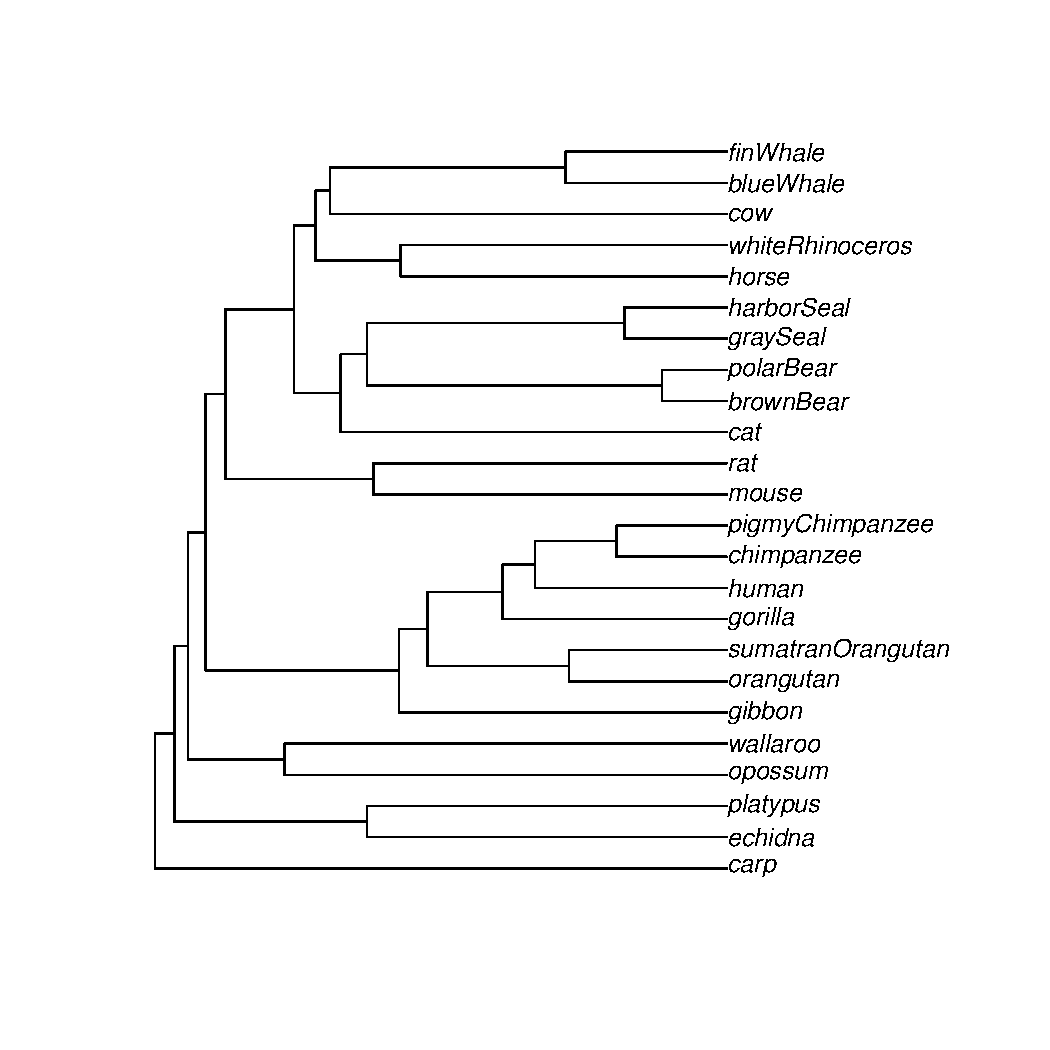
\includegraphics[scale=0.7]{24-mammals-average.pdf}
  \caption{Result of average linkage clustering of the distance matrix shown in table \ref{table:distance_matrix}. The height at which clusters join is proportional to the distance between them. }
  \label{figure:dendrogram_mammals}
\end{figure}

%% Chapter Template

\chapter{Classification} % Main chapter title

\label{Chapter4} % Change X to a consecutive number; for referencing this chapter elsewhere, use \ref{ChapterX}

\lhead{Chapter 4. \emph{Classification}}


Classification is a fundamental learning task. Given a training
set of objects for which the class is known, we want to identify the class
of an unknown object.

For example, we want to know if an incoming mail is \emph{spam}
(unsolicited message sent in bulk) or \emph{ham} (genuine message.) We
need an algorithm that extracts certain features from the incoming
message, compares it to features extracted from, say, a million messages
labeled as spam and a million labeled as ham, and decides to which class
it belongs.

Most real-world applications take a domain specific approach. Spam filters
count occurences of words and hyperlinks.

In this chapter, the normalized compression distance \eqref{ncd} is used
to extract features from objects. No domain knowledge is used. Then,
a support vector network is used to classify new data. The results are
compared to literature.  

\section{Classifying file fragments}

In forensics, file reconstruction is a big issue. Corrupted or wiped disks
may contain scattered fragments of files without metadata. File fragment
classification is a preliminary step in the reconstruction process.

The Govdocs1 dataset \cite{Garfinkel2009} is used throughout. It contains
nearly one million files of various types, acquired by querying search
egines with pseudo-random keywords.

Many authors, like \cite{Li2010}, \cite{Veenman2007} and
\cite{Axelsson2010}, try to classify compound file types (e.g. .doc or
.pdf.) Since a .ppt file may contain a .doc file, or a .pdf file may
contain a .jpg image, there is no way of telling the filetype of a 512 or
4096 byte block originating from such a file. If you misclassify .pdf as
     .jpg, did the classifier make a mistake, or did you stumble upon an
     embedded .jpg withing a .pdf? The answer is unknowable. This
     oversight is noted in \cite{Roussev2013}.

We will only use filetypes that are not compound, e.g. .html, .csv and
.jpg.

\subsection{Feature extraction}

Many statistical learning models, like artificial neural networks or
support vector machines, take as a training set fixed dimensional
vectors that correspond to a label:

\begin{equation}
  D = \{ (\vec{x_{i}}, y_{i}) \mid \vec{x_{i}} \in \mathbb{R}^{k}, i = 1, 2, \dots, n \}
\end{equation}

The mapping of actual objects onto feature vectors is the crucial step. In
\cite{Li2010}, byte frequencies are used as features, so $\vec{x_{i}}$ is
effectively a histogram, and $y_{i}$ is one of .dll, .exe, .pdf, .mp3,
.jpg. 

In \cite{Cilibrasi2007} a method is described to extract features from
objects using the normalized compression distance. For each file type,
(randomly) select some \emph{anchors} from the corpus of file fragments.
For simplicity, let's assume a binary classification problem of fragments
that are either from a .jpg or a .csv file. After picking 5 anchor
fragments for each type (totaling 10), we calculate the feature vector $\vec{x}$ for a file $f$ as follows:

\begin{equation}\label{}
  \vec{x} = ( NCD(f, a_{1}), NCD(f, a_{2}), \dots, NCD(f, a_{10}) )
\end{equation}

Table \ref{table:feature_vectors} shows an example feature vector of
a fragment for both file types. It becomes clear why a fragment can be
characterized this way: it's easy to see that the first fragment is a .csv
file, since it is close to the first five anchors (the .csv anchors.) .jpg
is a compressed format, so it has a distance of 1 from both the .csv and
.jpg anchors.

\begin{table}
\begin{tabular}{lrrrrrrrrrr}
\hline
 .csv & 0.91 & 0.94 & 0.94 & 0.86 & 0.95 & 1.01 & 1.00 & 1.01 & 1.02 & 1.02 \\
 .jpg & 1.01 & 1.01 & 1.01 & 1.01 & 1.01 & 1.00 & 1.00 & 1.00 & 1.00 & 1.00 \\
\hline
\end{tabular} \caption{Example feature vector for a .csv and a .jpg
fragment. The first five anchors are .csv fragments, the last five are
.jpg fragments. All fragments are randomly drawn from the Govdocs1
corpus.} \label{table:feature_vectors} \end{table}

\subsection{Support vector machine}

A support vector machine is a trainable binary classifier\footnote{A
classifier for more than two classes can be created from a combination of
binary classifiers, for example with a one-vs-rest strategy.}, first introduced in its current form in
\cite{Cortes1995}. For an extensive introduction, see \cite{Burges1998}.
In all experiments, I used the Python library scikit-learn
\cite{Pedregosa2011}, which uses \cite{Fan2014} and \cite{Chang2011}
internally.

In short, we want to separate the data points in the $d$-dimensional
feature space with a hyperplane that maximizes the margin (Euclidian
distance) to the closest data points. 

New data points fall on either side of the hyperplane and are classified
accordingly.

It is not possible to separate every set of points in all possible ways
with a linear function (i.e. a hyperplane.) You can show that hyperplanes
in $\mathbb{R}^{n}$ can, at most, separate $n + 1$ points in all possible
ways. So, if the training set is larger than the number of features plus
one, it may be inevitable that points in the training set are
misclassified by every hyperplane. The user-specified parameter $C$ weighs
the penalty for misclassified points in the training set. A higher value
of $C$ results in a hyperplane that misclassifies less training items.
(This may actually hurt the classifier's predictive power, a phenomenon
known as overfitting.) 

With some mathematical footwork (see \cite{Burges1998}), the optimization
problem can be formulated in terms of only the dot products $\langle
\vec{x_{i}}, \vec{x_{j}} \rangle$ of feature vectors. 

Nonlinear-classifiers can be created by replacing all dot products with
a \emph{kernel function} $k(\vec{x_{i}}, \vec{x_{j}})$. This effectively
applies a higher-dimensional transformation to the feature space.
A hyperplane is then constructed in that space, so that
non-separable data may become separable. This introduces extra parameters,
is more memory intensive and is prone to overfitting, but often gives
better results.

Two common kernel functions are the polynomial one

$$ k(\vec{x_{i}}, \vec{x_{j}}) = ( \langle \vec{x_{i}}, \vec{x_{j}}
\rangle + r )^{d} $$

which introduces parameters $r$ and $d$, and the radial basis
function (RBF)

$$ k(\vec{x_{i}}, \vec{x_{j}}) = e^{-\gamma ||\vec{x_{i}}
- \vec{x_{j}}||^{2}} $$

which introduces $\gamma$.

\subsection{Preparing the data set}


At the time of writing, it is possible to download samples of the Govdocs1
dataset \cite{Garfinkel2009}, called threads, of 1000 files each. I used
thread 0 through thread 7 as a corpus.

I created two corpora of fragmented files by chopping the files up into 512 or
4096 byte blocks, throwing away the first and last block of each file. The
     reasoning is that those blocks often contain header information, which is
     atypical for the file at large. It also ensures that all blocks are of
     equal size.

Table \ref{table:number_of_fragments} shows the number of fragments of each file type.

\begin{table}
\begin{tabular}{lr}
\hline
 File type   &   \# of fragments \\
\hline
 .csv        &                 47782 \\
 .jpg        &                 33630 \\
 .gz         &                 11507 \\
 .gif        &                 44367 \\
 .txt        &                 19539 \\
 .log        &                 25625 \\
 .xml        &                 9540  \\
 .html       &                 19934  \\
\hline
\end{tabular}
\caption{Number of 512-byte fragments per file type.}
\label{table:number_of_fragments}
\end{table}



\subsection{Training the classifier}

In each run of the experiment, randomly $n_{\text{anchors}}$ fragments per
filetype are selected as anchors, $n_{\text{training}}$ fragments per type are
selected as training data and $n_{\text{testing}}$ fragments per type are
selected as testing data.

\subsubsection{Scaling the feature vectors}

As is suggested in the scikit-learn documentation (\cite{Pedregosa2011}),
we rescale the features (the NCDs with the anchors) to have zero mean and
unit variance.


\subsubsection{Parameter estimation}

In \cite{Chih2008}, the authors describe a practical method for training
a support vector machine, and show that a simple grid search on the
classifier's parameters can dramatically improve results.

When using a radial basis function kernel, for example, we need to find
the best combination of $C$ and $\gamma$. First, we try all combinations
$ \{ (C, \gamma) \mid C, \gamma \in 2^{n}, n = -10, -9, \dots, 9, 10 \}$.
Then, after the best $C$ and $\gamma$ in that grid have been determined,
we can perform successively more precise estimations by forming a finer
grid around the current optimum.

The fitness of the parameters is assessed by $k$-fold cross validation.
The training set is partitioned into $k$ chunks of equal size. $k - 1$
chunks are used as training data and the remaining chunk as test data. In
$k$ runs, every chunk is used once as test data. The results are averaged.

\subsection{Experiments}

\subsubsection{Classifying .csv and .jpg fragments}

As a sanity check, we classify .csv and .jpg fragments. They should be
easily distinguishable, since .jpg has high entropy (it is a compressed
format) and .csv is very regular. Table \ref{table:csv_jpg_recall} shows
this to be the case. The recall rate is almost perfect, and it doesn't
seem to depend on the amount of anchors per type.

\begin{table}[h]
\begin{tabular}{rrr}
\hline
   anchors/type &   .csv recall \% &   .jpg recall \% \\
\hline
             10 &           99.96 &           99.52 \\
              5 &           99.84 &           99.76 \\
              2 &           99.88 &           99.34 \\
\hline
\end{tabular}
\caption{
The results were acquired by averaging recall rates over five
independent runs. In each run, 1000 distinct training fragments and 500
distinct test fragments per file type were selected. After feature
extraction, the support vector machine with an RBF kernel was trained by doing a grid search
for $C \in \{ 2^{1}, 2^{2}, \dots, 2^{9} \}$ and $\gamma \in \{2^{-8},
2^{-7}, \dots, 2^{0} \}$, optimized for the training set with a two-fold
cross validation. All fragments are 512 bytes.}
\label{table:csv_jpg_recall}
\end{table}

\subsubsection{Classifying .gz and .jpg fragments}

Now, we train the classifier on two compressed formats. The recall rate is
very bad and .jpg gets many false positives. Training on .gif and .mp3
instead of .gz gives similar results. Increasing the training set from 1000 to 10000 sample fragments per type doesn't improve results, either.

\begin{table}[h]
\begin{tabular}{rrr}
\hline
   anchors/type &   .gz recall \% &   .jpg recall \% \\
\hline
             10 &           31.24 &           96.76 \\
              2 &           19.52 &           96.84 \\
\hline
\end{tabular}
\caption{
The results were acquired by averaging recall rates over five
independent runs. In each run, 1000 distinct training fragments and 500
distinct test fragments per file type were selected. The kernel is RBF, $C
\in \{ 2^{-3}, 2^{2}, \dots, 2^{9} \}$ and $\gamma \in \{2^{-8}, 2^{-7},
\dots, 2^{4} \}$, optimized for the training set with a two-fold cross
validation. All fragments are 512 bytes.} \label{table:gz_jpg_recall}
\end{table}



\subsubsection{Classifying .csv, .html, .jpg and .log}

Table \ref{table:csv_html_jpg_log_recall} shows that classification still
works very well on four different file types of low entropy. Note that
adding more anchors now significantly improves results.


\begin{table}[h]
\begin{tabular}{rrrrr}
\hline
   anchors/type &   .csv recall \% &   .html recall \% &   .jpg recall \% &   .log recall \% \\
\hline
              2 &           94.00    &            92.32 &           98.84 &           87.28 \\
             10 &           98.48 &            95.04 &           99.12 &           95.24 \\
\hline
\end{tabular}
\caption{
The results were acquired by averaging recall rates over five
independent runs. In each run, 1000 distinct training fragments and 500
distinct test fragments per file type were selected. The kernel is RBF, $C
\in \{ 2^{0}, 2^{1}, \dots, 2^{5} \}$ and $\gamma \in \{2^{-7}, 2^{-6},
\dots, 2^{-1} \}$, optimized for the training set with a two-fold cross
validation. All fragments are 512 bytes.}
\label{table:csv_html_jpg_log_recall}
\end{table}
 
%% Chapter 1

\chapter{Conclusion} % Main chapter title

\label{Conclusion} % For referencing the chapter elsewhere, use \ref{Chapter1}

\lhead{\emph{Conclusion}} % This is for the header on each page - perhaps a shortened title

HoiHoi blaf
 
%\input{Chapters/Chapter6} 
%\input{Chapters/Chapter7} 

%----------------------------------------------------------------------------------------
%	THESIS CONTENT - APPENDICES
%----------------------------------------------------------------------------------------

%\addtocontents{toc}{\vspace{2em}} % Add a gap in the Contents, for aesthetics
%
%\appendix % Cue to tell LaTeX that the following 'chapters' are Appendices
%
%% Include the appendices of the thesis as separate files from the Appendices folder
%% Uncomment the lines as you write the Appendices
%
%% Appendix A

\chapter{Appendix Title Here} % Main appendix title

\label{AppendixA} % For referencing this appendix elsewhere, use \ref{AppendixA}

\lhead{Appendix A. \emph{Appendix Title Here}} % This is for the header on each page - perhaps a shortened title

Write your Appendix content here.
%%\input{Appendices/AppendixB}
%%\input{Appendices/AppendixC}
%
%\addtocontents{toc}{\vspace{2em}} % Add a gap in the Contents, for aesthetics

\backmatter

%----------------------------------------------------------------------------------------
%	BIBLIOGRAPHY
%----------------------------------------------------------------------------------------

\label{Bibliography}

\lhead{\emph{Bibliography}} % Change the page header to say "Bibliography"

\bibliographystyle{unsrtnat} % Use the "unsrtnat" BibTeX style for formatting the Bibliography

\bibliography{library} % The references (bibliography) information are stored in the file named "Bibliography.bib"

\end{document}  